\documentclass{article}
\usepackage[utf8]{inputenc}
\usepackage{geometry}
\usepackage{amsmath}
\usepackage{url}
\usepackage[utopia]{mathdesign}
\usepackage{lipsum}  
\usepackage{lmodern}
\usepackage{listings}

 \geometry{
 a4paper,
 total={170mm,257mm},
 left=20mm,
 top=20mm,
 }
 \usepackage{graphicx}
 \usepackage{titling}

 \title{Simulation of the dynamic motion of a pendulum under viscous friction with Cartesian coordinates
}
\author{GU JUN}
\date{October 23, 2024}
 
 \usepackage{fancyhdr}
\fancypagestyle{plain}{%  the preset of fancyhdr 
    \fancyhf{} % clear all header and footer fields
%    \fancyfoot[R]{\includegraphics[width=5cm]{}}
    \fancyfoot[L]{\today}
    \fancyhead[L]{Analytical Mechanics 80848\#1}
    \fancyhead[R]{HIRAI SHINCHI}
}
\makeatletter
\renewcommand{\maketitle}{%
  \newpage
  \null
  \vskip 1em%
  \begin{center}%
  \let \footnote \thanks
    {\LARGE \@title \par}%
    \vskip 1em%
    %{\large \@date}%
  \end{center}%
  \par
  \vskip 1em}
\makeatother


\begin{document}

\maketitle

\noindent\begin{tabular}{@{}ll}
    Student & \theauthor\\
    ID number & 6132230056 \\
\end{tabular}

\section*{Problem Statement}
Simulate the dynamic motion of a pendulum under viscous friction
described with Cartesian coordinates x and y.
Apply constraint stabilization method to convert the constraint into its almost
equivalent ODE, then apply any ODE solver to solve a set of ODEs
(equations of motion and equations for constraint stabilization)
numerically.

% \begin{figure}
%     \centering
%     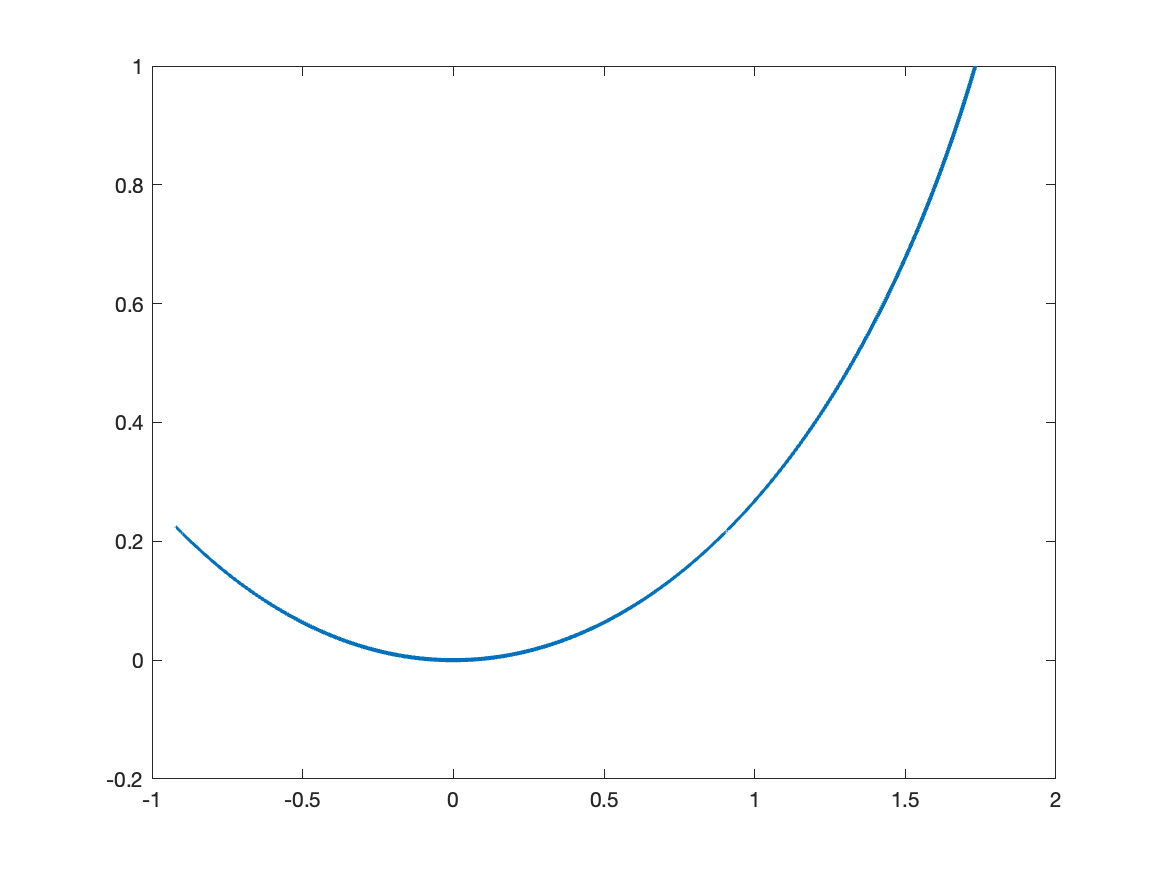
\includegraphics[width=0.6\linewidth]{pendulum_Cartesian_path.png}
%     \caption{Simulation of the dynamic motion of a pendulum under viscous friction with Cartesian coordinates.}
%     \label{fig:enter-label}
% \end{figure}

\section*{Dynamic analysis}
According to previous content about viscous friction, the equation of the viscous friction is given by:
\begin{equation}
    \tau = -b\mathbf{\dot{\theta}}
\end{equation}
where $\tau$ is the torque, $b$ is the viscous friction coefficient, and $\mathbf{\dot{\theta}}$ is the angular velocity.\\
We can easily get the equation of motion under Cartesian coordinates:
\begin{equation}
    f_v = -\frac{b}{l} v
\end{equation}
where $f_v$ is the force, $b$ is the viscous friction coefficient, $l$ is the length of the pendulum, and $v$ is the velocity.\\
Then we can get the equations for $x$ and $y$:
\begin{equation}
    \left[\begin{array}{c}
    f_x \\
    f_y
    \end{array}\right] = -\frac{b}{l} \left[\begin{array}{c}
    \dot{x} \\
    \dot{y}
    \end{array}\right]
  \end{equation}
where $f_x$ and $f_y$ are the viscous forces in $x$ and $y$ directions, respectively.\\
Treat the viscous forces as external forces, and use the above equations in the system that described in the sides.
we can get the equations of motion:
\begin{equation}
  \label{eq:dynamic}
  \begin{aligned}
  \dot{x} & =v_x \\
  \dot{y} & =v_y \\
  {\left[\begin{array}{ccc}
  m & & -R_x \\
  & m & -R_y \\
  -R_x & -R_y
  \end{array}\right]\left[\begin{array}{c}
  \dot{v}_x \\
  \dot{v}_y \\
  \lambda
  \end{array}\right] } & =\left[\begin{array}{c}
  f_x \\
  -m g+f_y \\
  C\left(x, y, v_x, v_y\right)
  \end{array}\right]
  \end{aligned}
\end{equation}
where $m$ is the mass of the pendulum, $g$ is the acceleration of gravity, $\lambda$ is the Lagrange multiplier, $R_x$ and $R_y$ are the constraint forces in $x$ and $y$ directions, respectively.\\
$C\left(x, y, v_x, v_y\right)$ is the constraint function, which is given by:
\begin{equation}
  \begin{aligned}
  C\left(x, y, v_x, v_y\right) & =\left[\begin{array}{ll}
  v_x & v_y
  \end{array}\right]\left[\begin{array}{ll}
  R_{x x} & R_{x y} \\
  R_{y x} & R_{y y}
  \end{array}\right]\left[\begin{array}{l}
  v_x \\
  v_y
  \end{array}\right] \\
  & +2 \alpha\left(R_x v_x+R_y v_y\right)+\alpha^2 R
  \end{aligned}
  \end{equation}
where $\alpha$ is a constant, and $R$ is the distance between the pendulum and the constraint.\\
$R_x$, $R_y$, $R_{x x}$, $R_{x y}$, $R_{y x}$, and $R_{y y}$ are the derivatives of $R$ with respect to $x$ and $y$.\\
With Equation~\ref{eq:dynamic}, we can start our simulation in MATLAB.
\newpage
\section*{MATLAB code}
The code of modified part is shown below:
\begin{center}
\begin{lstlisting}[language=Matlab, caption={MATLAB code for pendulum simulation}, basicstyle=\small\ttfamily]
function dotq = pendulum_cartesian (t,q)
  global mass; global length; global grav; global alpha; global viscous_coeiff;
  x = q(1); y = q(2); vx = q(3); vy = q(4);
  
  dotx = vx; doty = vy;
  R = sqrt(x^2+(y-length)^2) - length;
  P = 1/sqrt(x^2+(y-length)^2); Rx = x*P; Ry = (y-length)*P;
  Rxx = P - x^2*P^3; Ryy = P - (y-length)^2*P^3;
  Rxy = -x*(y-length)*P^3;
  C = [vx,vy]*[Rxx, Rxy; Rxy, Ryy]*[vx;vy] ...
    + 2*alpha*(Rx*vx + Ry*vy) ...
    + alpha^2*R;
  A = [mass, 0, -Rx; 0, mass, -Ry; -Rx, -Ry, 0];
  \textcolor{red}{b = [ -viscous_coeiff*dotx; -mass*grav - viscous_coeiff*doty; C ];}

  s = A \ b;
  dotvx = s(1); dotvy = s(2);
  dotq = [dotx; doty; dotvx; dotvy];
end
\end{lstlisting}
\end{center}
Using ode45 function in MATLAB, we can solve the ODEs numerically.\\
\section*{Results}
Using the following parameters: mass of 0.01 kg, length of 2.0 m, gravitational acceleration of 9.8 m/s², alpha of 1000, viscous coefficient of 0.01, initial angle of $\frac{\pi}{3}$ radians, and a simulation time of 10 seconds, we can obtain the simulation results as shown below:
\begin{figure}[h]
  \centering
  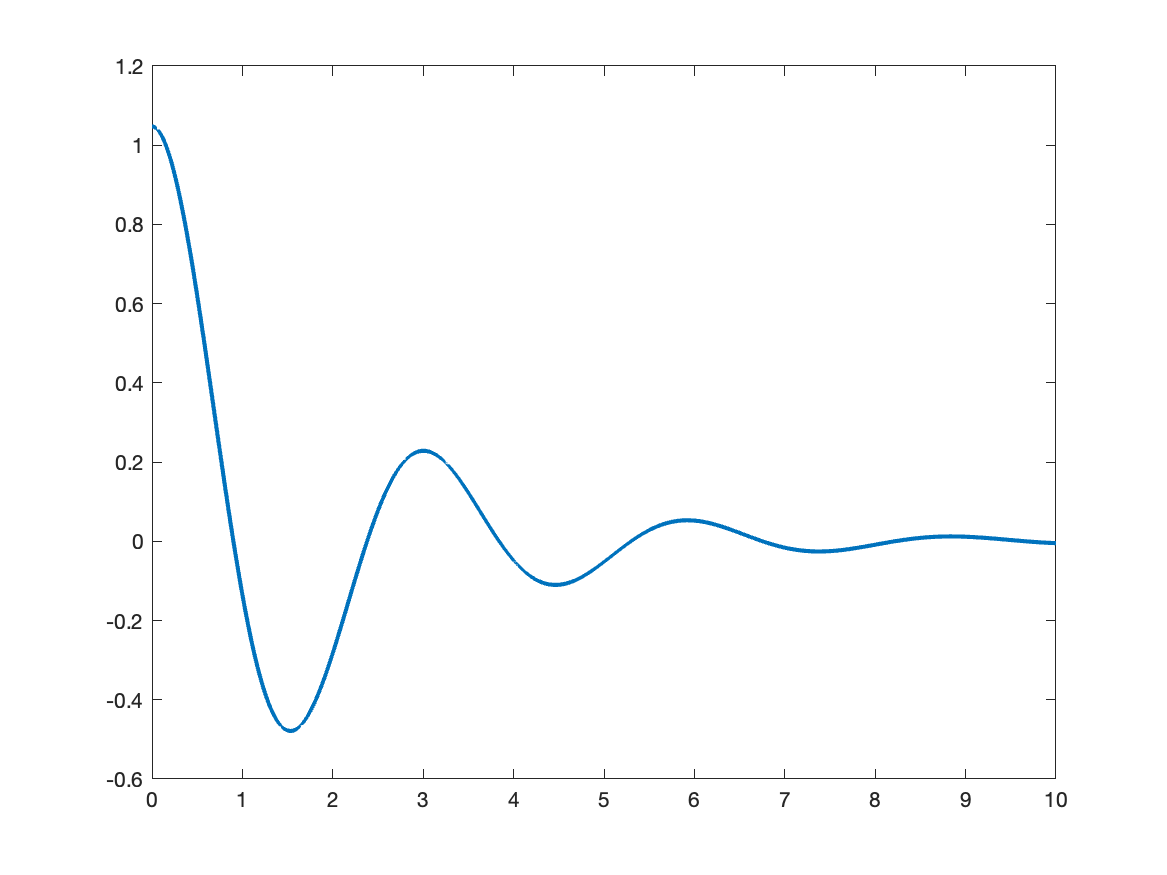
\includegraphics[width=0.3\linewidth]{pendulum_Cartesian_computed_angle.png}
  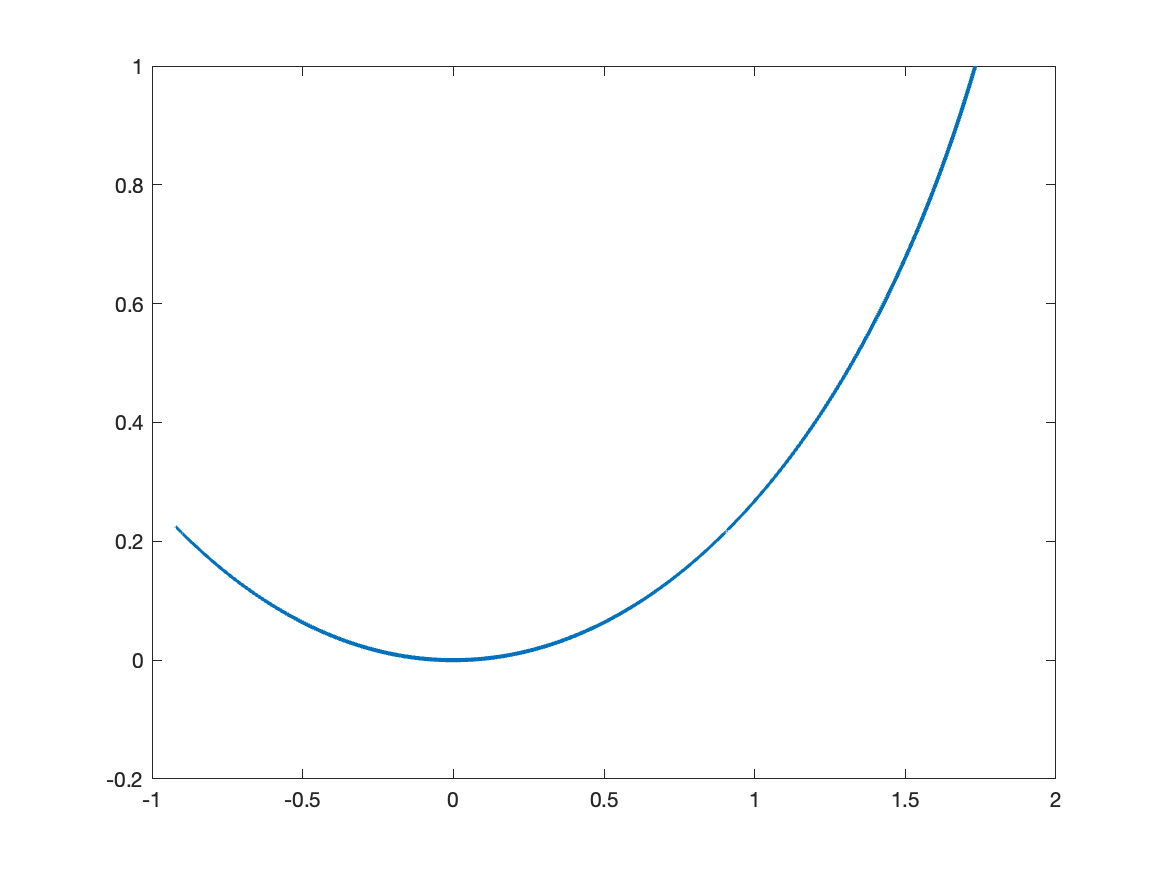
\includegraphics[width=0.3\linewidth]{pendulum_Cartesian_path.png}
  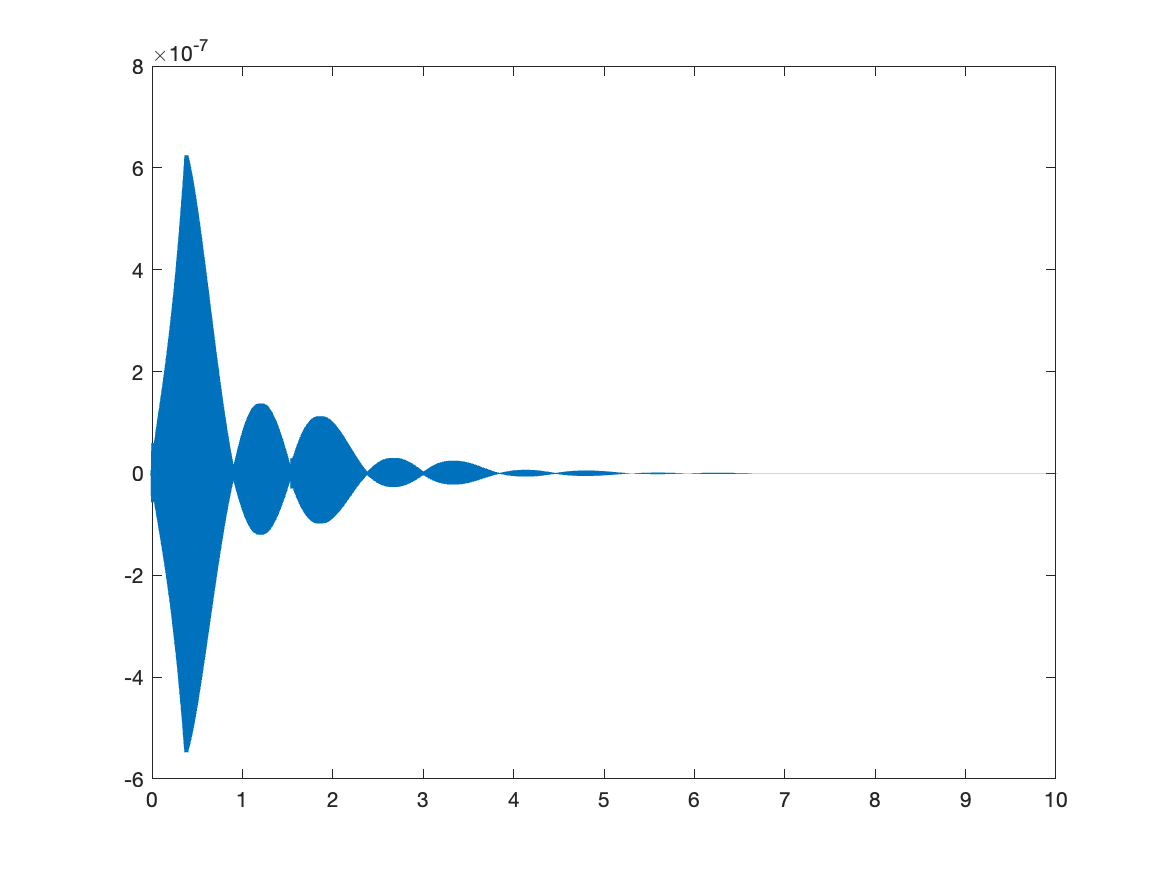
\includegraphics[width=0.3\linewidth]{pendulum_Cartesian_R.png}
  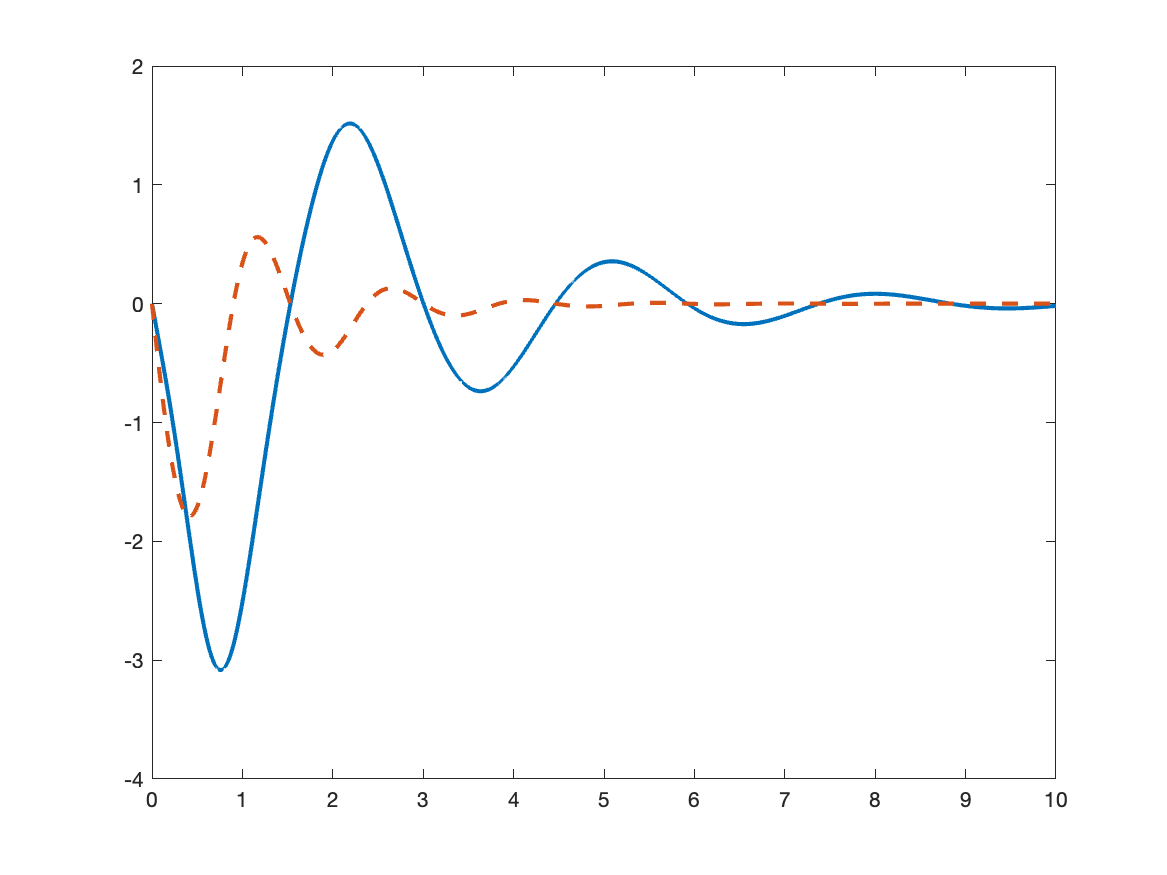
\includegraphics[width=0.3\linewidth]{pendulum_Cartesian_vx_vy.png}
  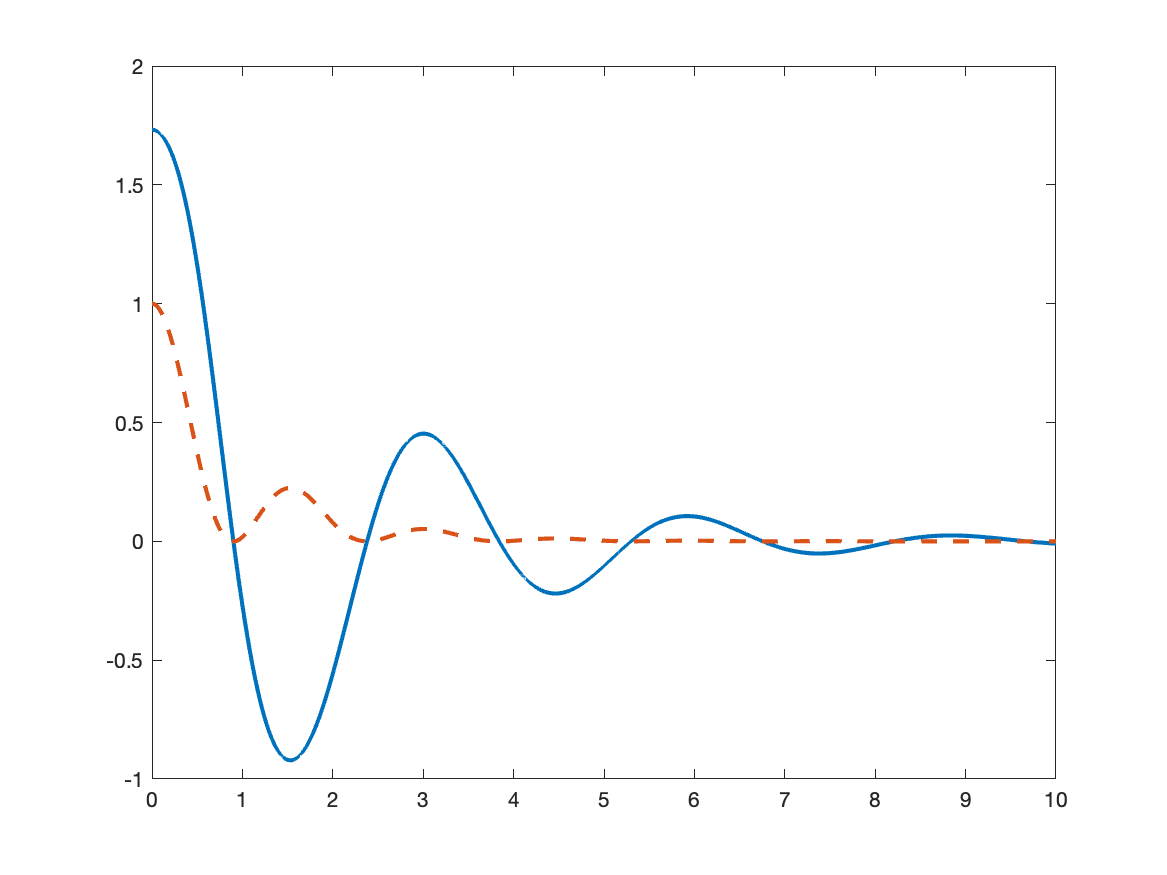
\includegraphics[width=0.3\linewidth]{pendulum_Cartesian_x_y.png}
  \caption{(a) Computed angle of the pendulum, (b) Path of the pendulum, (c) Distance R between the pendulum and the constraint, (d) Velocities $v_x$ and $v_y$, (e) Positions $x$ and $y$ of the pendulum.(a) - (e) are ordered from left to right and top to bottom.}
  \label{fig:pendulum_simulation}
\end{figure}

\end{document}
